\documentclass[10pt]{beamer}

\usetheme[progressbar=frametitle]{metropolis}
\usepackage{appendixnumberbeamer}

\usepackage{booktabs}
\usepackage[scale=2]{ccicons}

\usepackage{pgfplots}
\usepgfplotslibrary{dateplot}

\usepackage{xspace}
\newcommand{\themename}{\textbf{\textsc{metropolis}}\xspace}

\hypersetup{
    colorlinks=true,
    linkcolor=blue,
    filecolor=magenta,      
    urlcolor=cyan,
}

\title{MIT Spotlight}
\subtitle{Strangers in a Strange Land}
% \date{\today}
\date{December 6}
\author{Diego Roque}
\institute{MIT}
% \titlegraphic{\hfill\includegraphics[height=1.5cm]{logo.pdf}}

\begin{document}

\maketitle

\begin{frame}{Table of contents}
  \setbeamertemplate{section in toc}[sections numbered]
  \tableofcontents[hideallsubsections]
\end{frame}

\section{Introduction}

\begin{frame}[fragile]{Statistics}

International students at MIT make 
around 10\% of the undergraduate population, 40\% of the graduate population. Qualitatively, my living group is mostly non-Americans 
or Americans raised abroad.

They are not \textit{explicitly} captured by spotlights.

\end{frame}

\section{Exigence and Designing}

\begin{frame}{Constraints}

On the other hand, 90\% of the undergraduate population is American,
and MIT is an American institution. Moreover, MIT is funded by
American taxpayers. How to capture the international 
experience without alienating the general population? Should it be 
captured at all?

\end{frame}

\begin{frame}{Exigence, Again}

\begin{center}
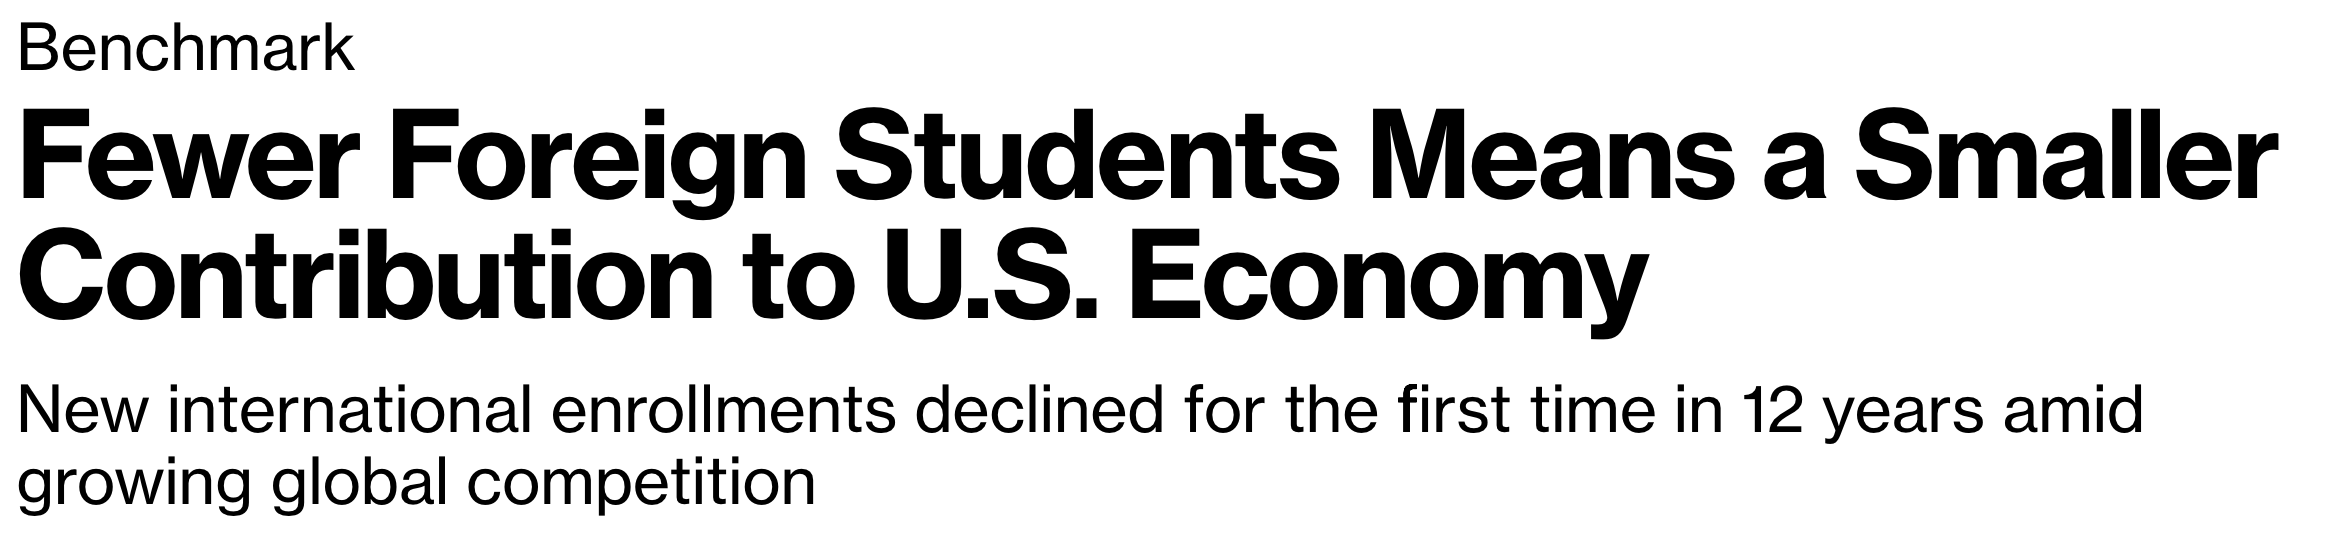
\includegraphics[scale=0.2]{fewer_foreign.png}
\end{center}


\begin{center}
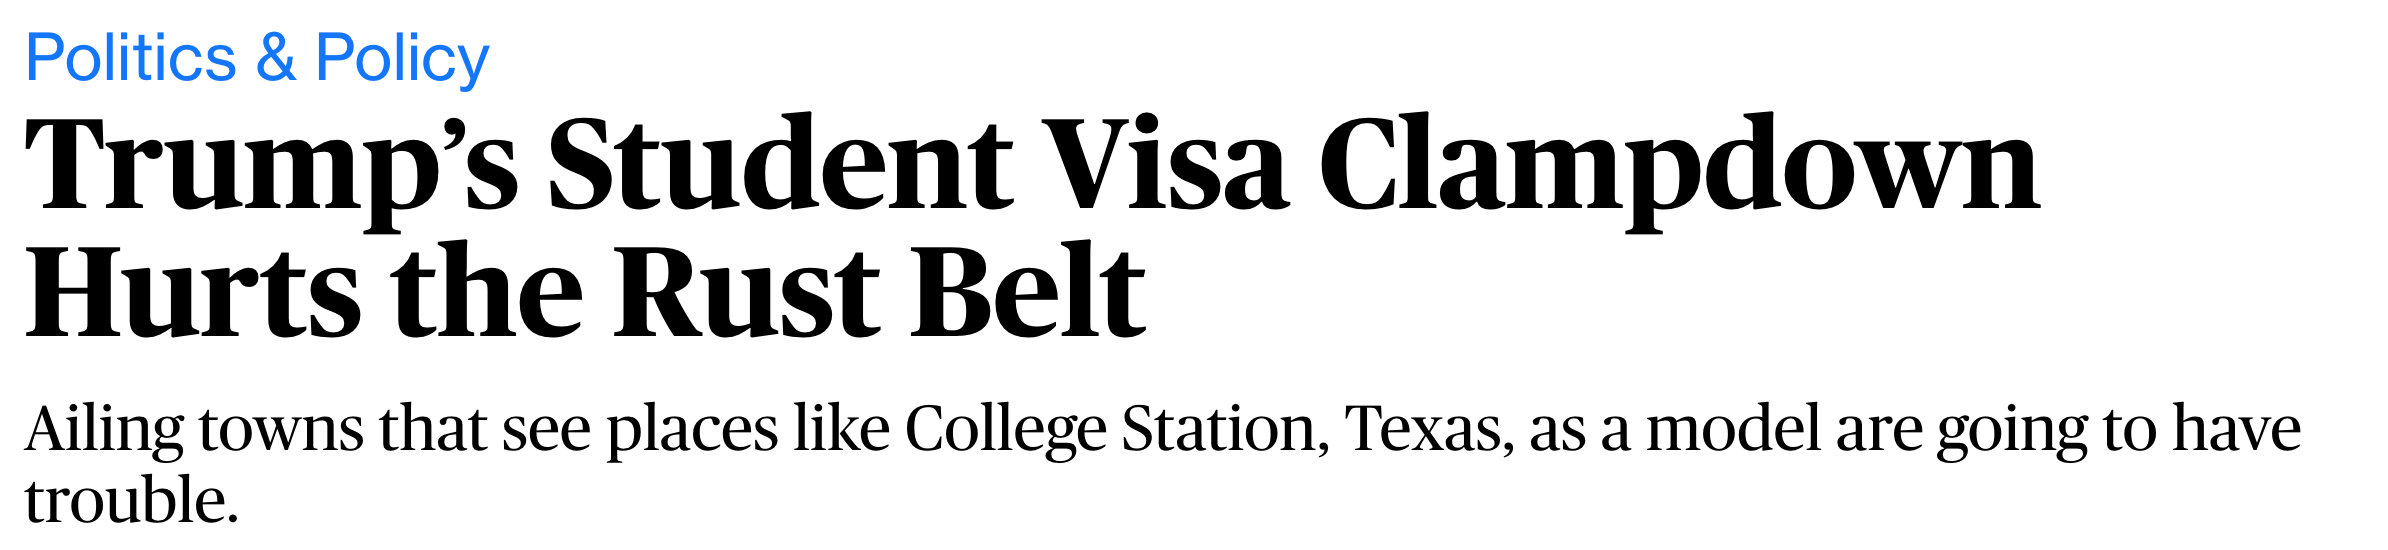
\includegraphics[scale=0.2]{rust_belt_visa.png}
\end{center}

\end{frame}

\begin{frame}{Constraints, Again}

\begin{itemize}
  \item No political stuff. Too divisive between Americans. It would risk a PR problem 
  and it wouldn't be helpful. 
  \item Relatable to Americans at large, not only "liberal pockets".
  \item No visa stuff. Too political and not relatable.
\end{itemize}

\end{frame}

\begin{frame}{Idea}

MIT Thanksgiving's spotlight is \textbf{bad}. 
Thanksgiving is a very American thing, and most Americans (who can afford it)
travel back to spend it with their families. 

International students still get the break, but it's more expensive to travel
and there's no real reason to.

We can use this as the base for the spotlight. 

\end{frame}


\section{Elements}


\begin{frame}{Central photo}

\begin{center}
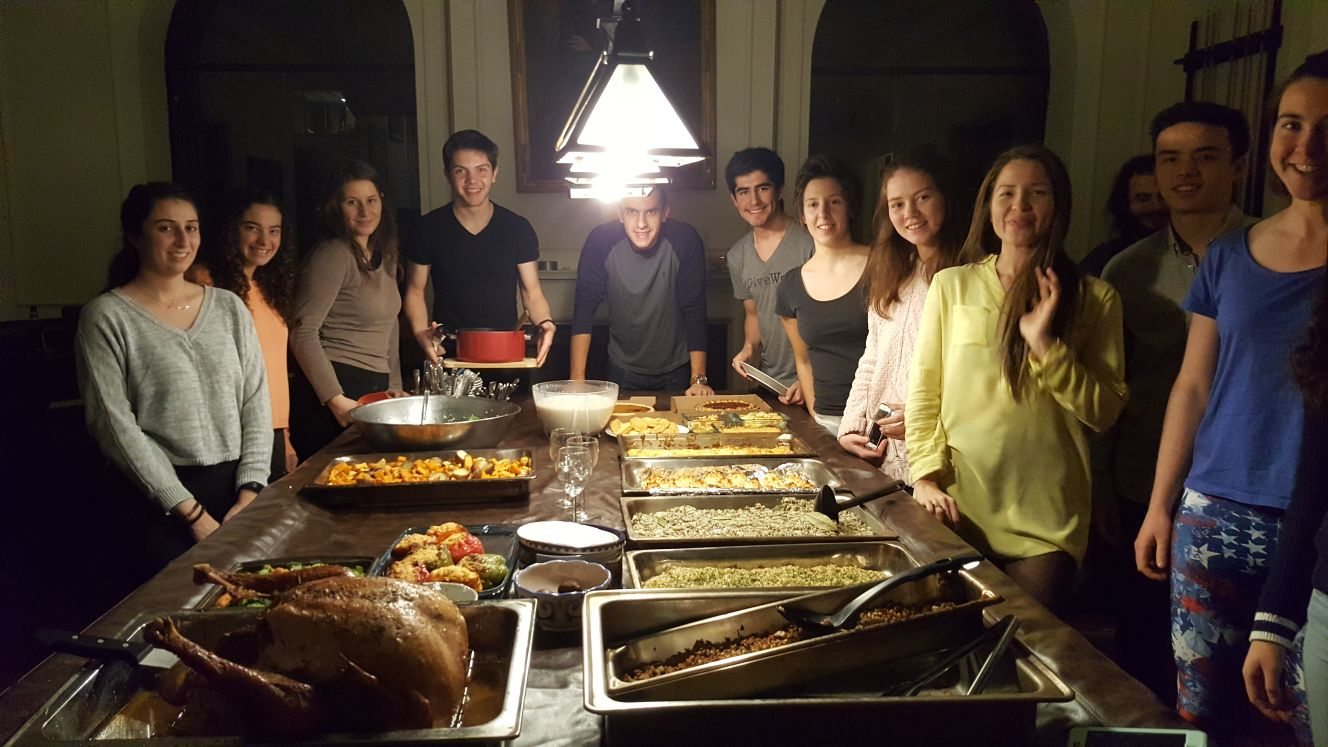
\includegraphics[scale=0.20]{Thanksgiving_2017.jpeg}
\end{center}

\end{frame}

\begin{frame}{What can we extract?}

Most of the food in the photo are plates that students eat in their home countries.
To be concrete, 11 international students and one american student. 
It still contains some food served traditionally in Thanksgiving.
Few, but some, of the people in the picture had actually been in a "real" Thanksgiving. 
Internationals in America parallel the Pilgrims in the new world.


\end{frame}

\begin{frame}{Accompanying text}

Like many \href{http://iso.mit.edu}{international students}, members of the highly
international \href{http://no6.mit.edu}{Number Six} stay at MIT during Thanksgiving and celebrate
a tradition that is new for them.

The link to the full story would be "Strangers in a Strange Land: Celebrating 
Thanksgiving as an International Student".

\end{frame}

\begin{frame}{Website}

\begin{center}
  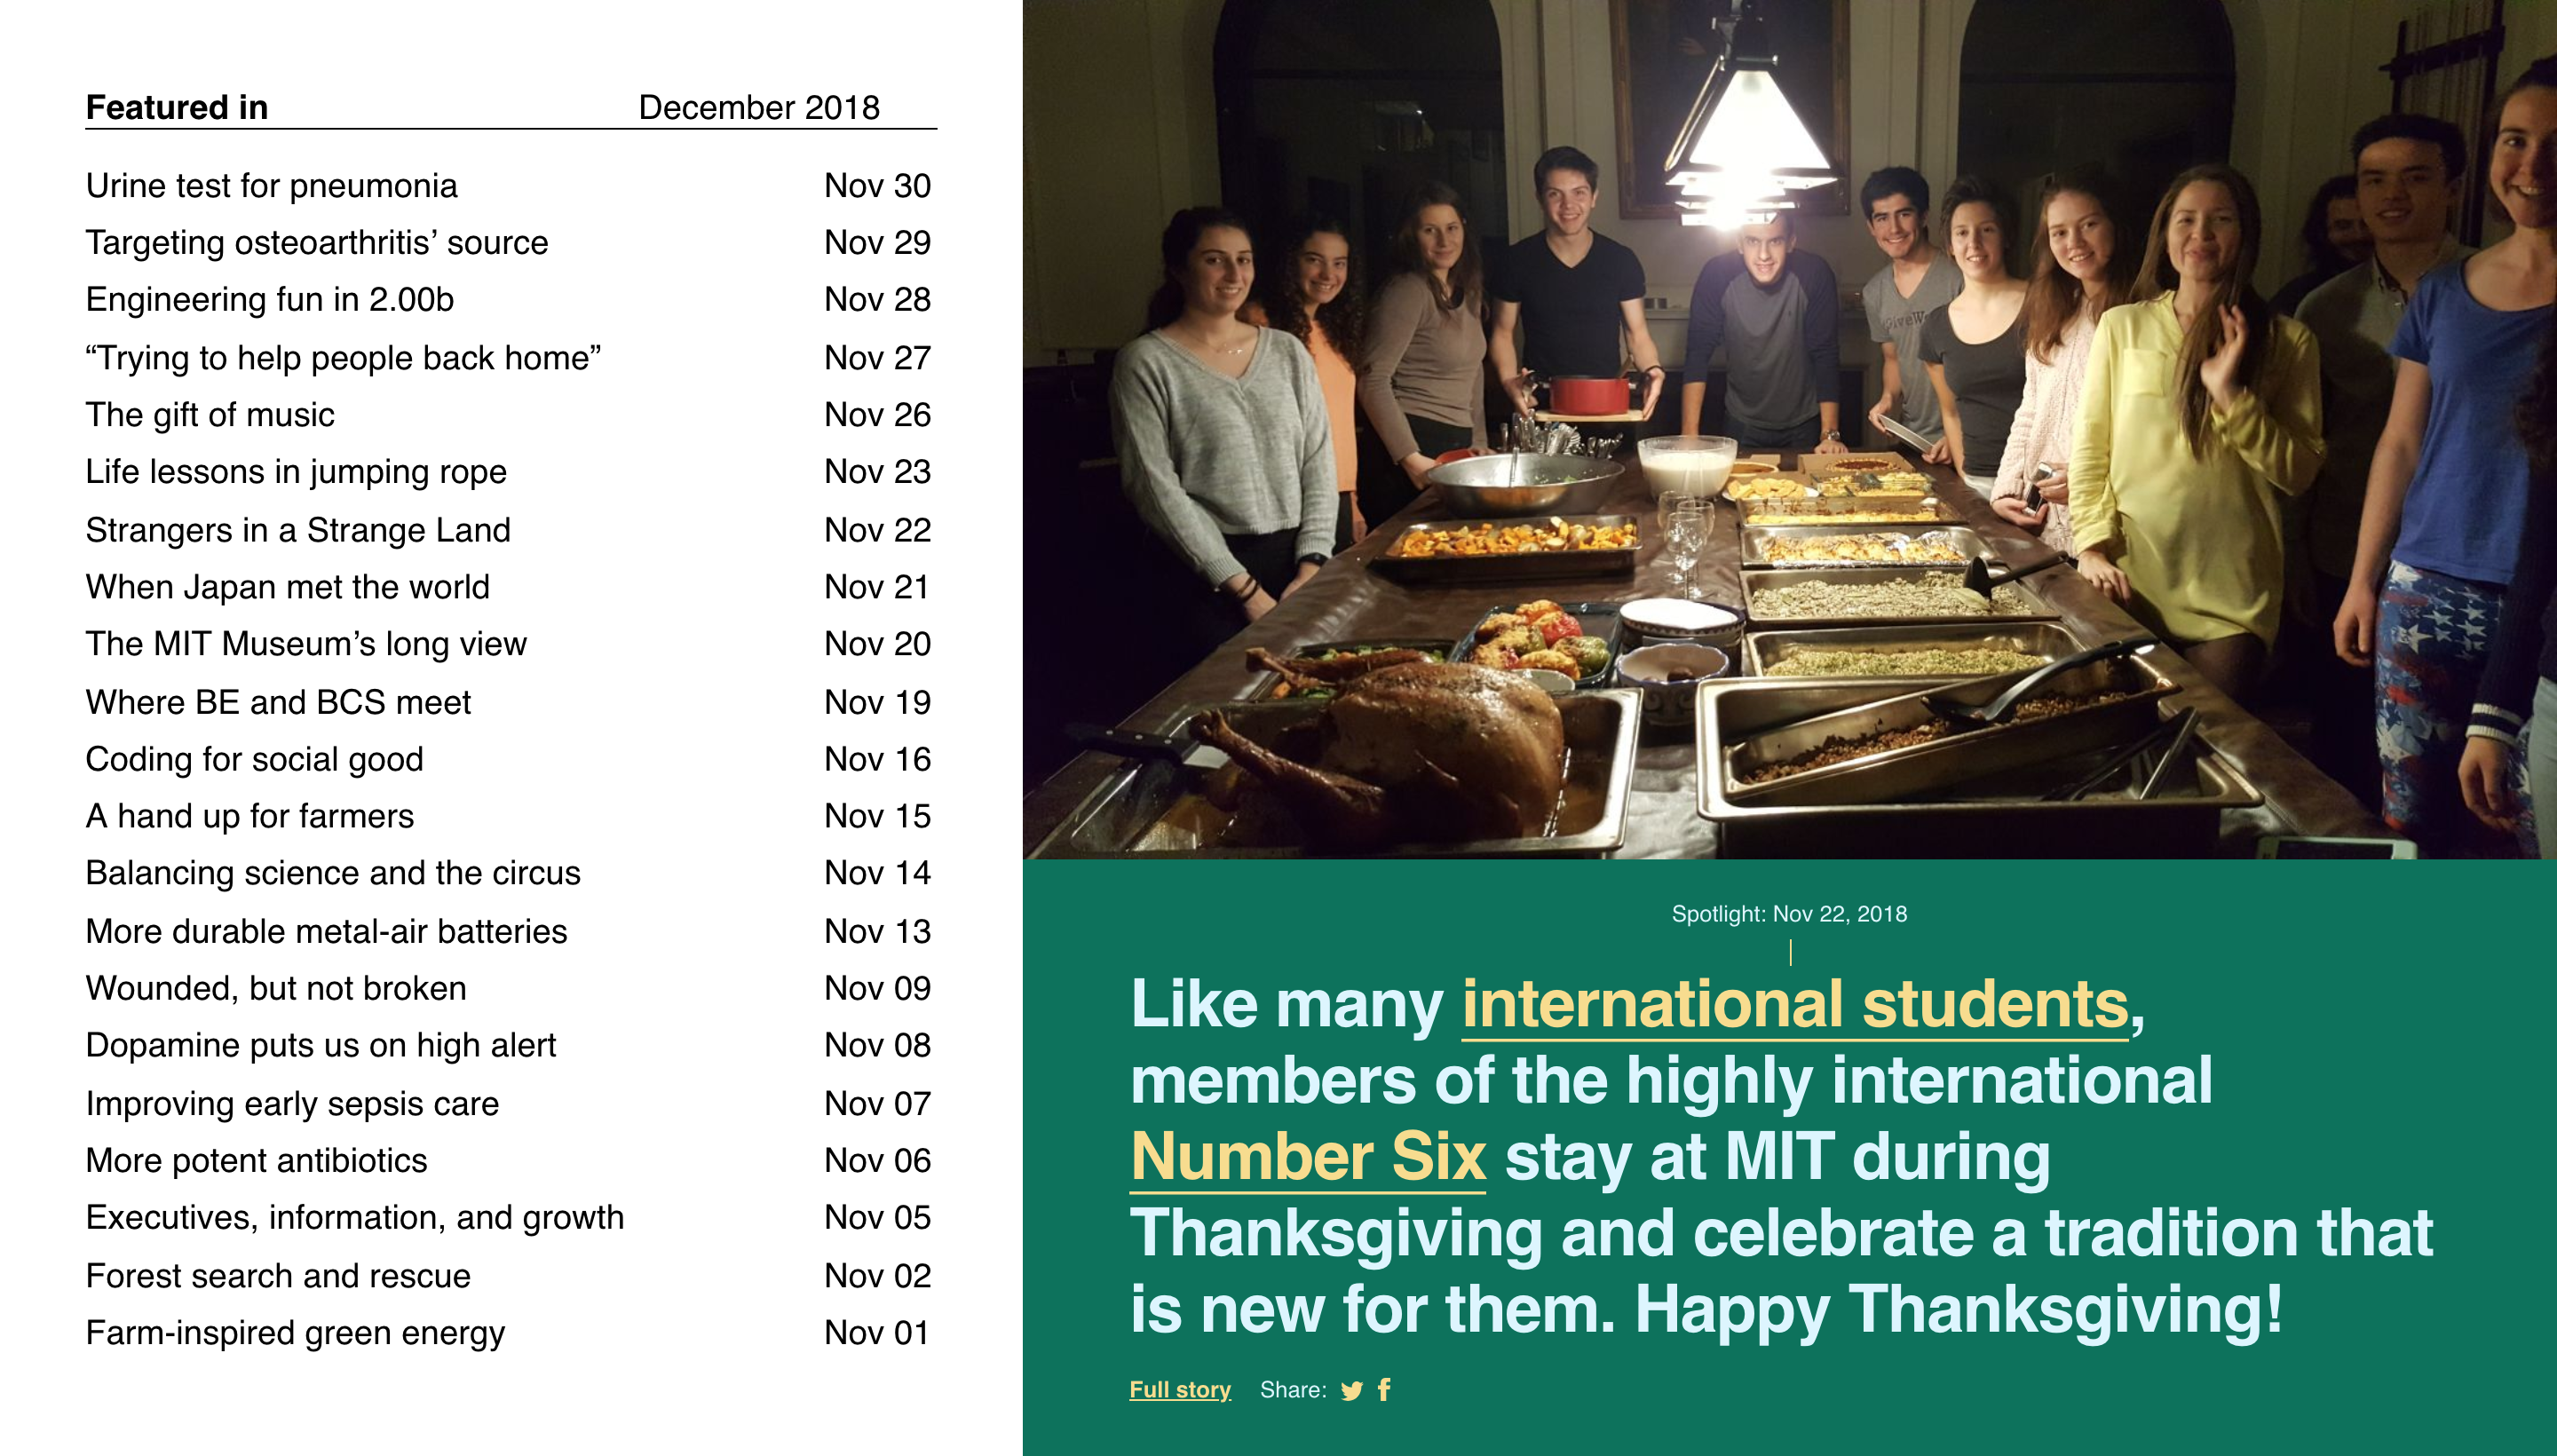
\includegraphics[scale=0.2]{Thanksgiving_website.png}
\end{center}

\end{frame}

\begin{frame}{Connotations}


Thanksgiving hence it's a good option because it's very recognizable, because of the 
already existing connotations of people in a new place.

People outside MIT will understand the general scene.
Americans will be familiar, internationals will be happy to know they will have a 
community in this new place.

\end{frame}


\begin{frame}{References}
  \cite{ndugga_2017, smith_2018}
\end{frame}

\section{Conclusion}

{\setbeamercolor{palette primary}{fg=black, bg=yellow}
\begin{frame}[standout]
  Questions?
\end{frame}
}

\appendix


\begin{frame}[allowframebreaks]{References}

  \bibliography{demo}
  \bibliographystyle{abbrv}

\end{frame}

\end{document}
